\begin{frame}{Լրիվ գրաֆների միջակայքային ներկումներ}
\begin{itemize}
    \item Լրիվ գրաֆը ունի միջակայքային ներկում այն և միայն այն դեպքում, երբ գագաթների քանակը զույգ է:
    \item $w(K_{2n})=2n-1$:
    \item $W(K_{2n})$-ի գնահատականներ ստացել են Քամալյանը (1990), Գիառոն, Կուբալը և Մալաֆիյսկին (2001) և Պետրոսյանը (2010):
\end{itemize}

\end{frame}


\begin{frame}[shrink]{$1$-ֆակտորիզացիա}

$\mathfrak{F} = \left\{F_1,\ldots,F_n \right\}$ կատարյալ զուգակցումների բազմությունը կանվանենք $G$ մուլտիգրաֆի $1$-ֆակտորիզացիա, եթե $G$-ի կամայական կող պատկանում է $\mathfrak{F}$-ի զուգակցումներից ճիշտ մեկին:

\begin{figure}[t!]
\centering
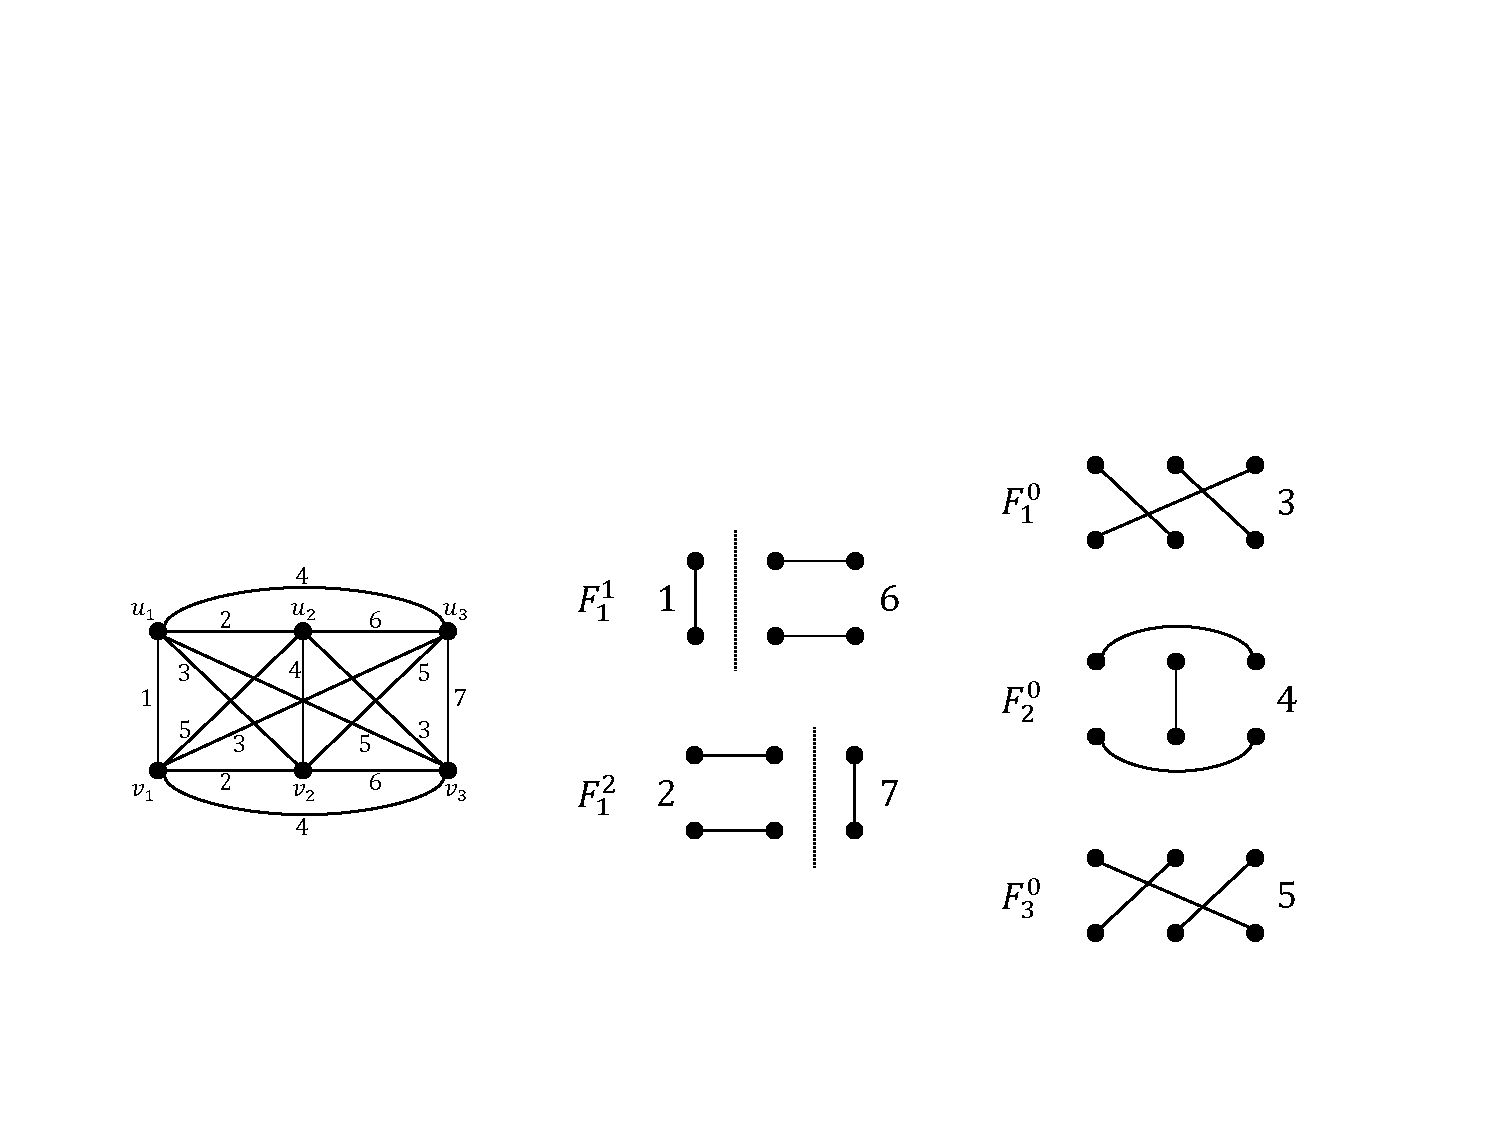
\includegraphics[width=0.9\textwidth]{figures/K_6factorization.pdf}
\label{K_6factorization}
\end{figure}
\end{frame}


\begin{frame}[shrink]{Միջակայքային ներկումների և ֆակտորիզացիայի համարժեքությունը լրիվ գրաֆների համար}

\begin{itemize}
\item Ֆիքսենք գագաթների համարակալում. $\mathbf{v} = \left(u_1,v_1, u_2,v_2, \ldots,u_n,v_n\right)$ 
\item $F$ կատարյալ զուգակցումը կանվանենք \textbf{$i$-բաժանված} ($\mathbf{v}$ համարակալման նկատմամբ), եթե զուգակցման կողերը կարելի է տրոհել երկու մասի այնպես, որ մի մասը ծածկեն $u_1, v_1, \ldots, u_i, v_i$ գագաթները, իսկ մյուս մասը՝ $u_{i+1}, v_{i+1}, \ldots, u_n, v_n$ գագաթները:
\end{itemize}


\begin{figure}[t!]
\centering
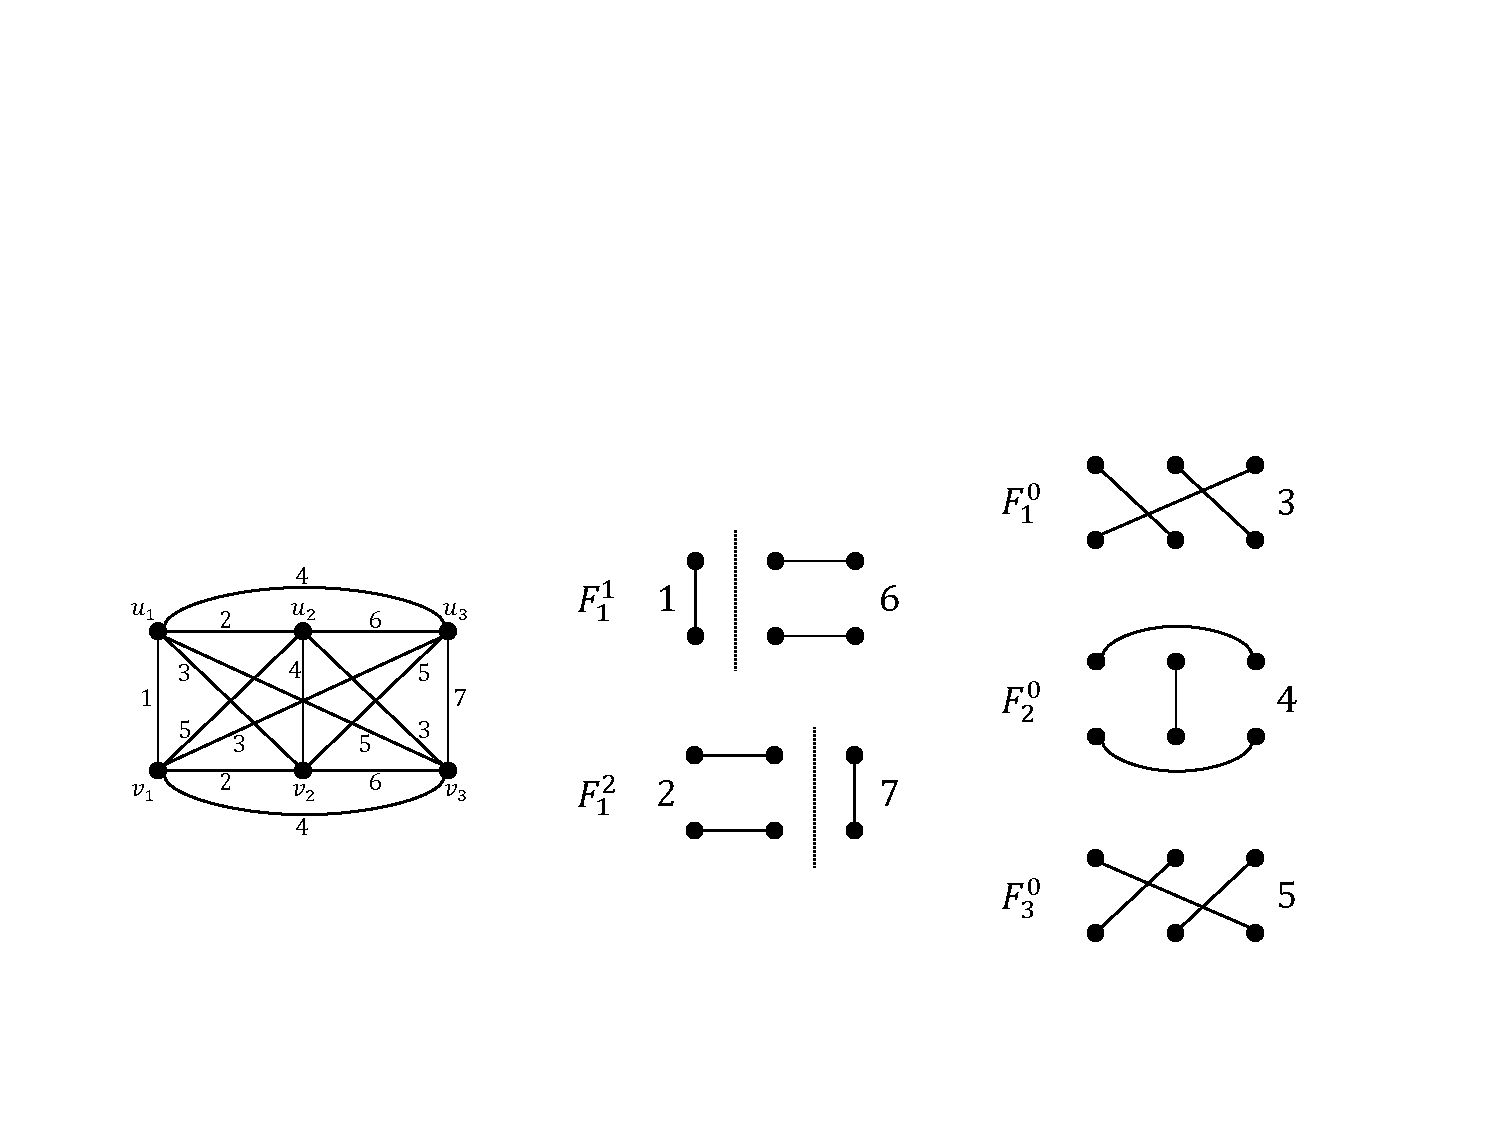
\includegraphics[width=0.7\textwidth]{figures/K_6factorization.pdf}
\label{K_6factorization}
\end{figure}
\end{frame}

\begin{frame}{Միջակայքային ներկումների և ֆակտորիզացիայի համարժեքությունը լրիվ գրաֆների համար}

\begin{theorem}[1.3.12]
Ցանկացած $n\in\mathbb{N}$-ի համար $K_{2n}$-ը ունի միջակայքային $t$-ներկում այն և միայն այն դեպքում, երբ այն ունի այնպիսի $1$-ֆակտորիզացիա, որտեղ առնվազն $t-2n+1$ կատարյալ զուգակցումներ բաժանված են:
\end{theorem}

\begin{figure}[t!]
\centering
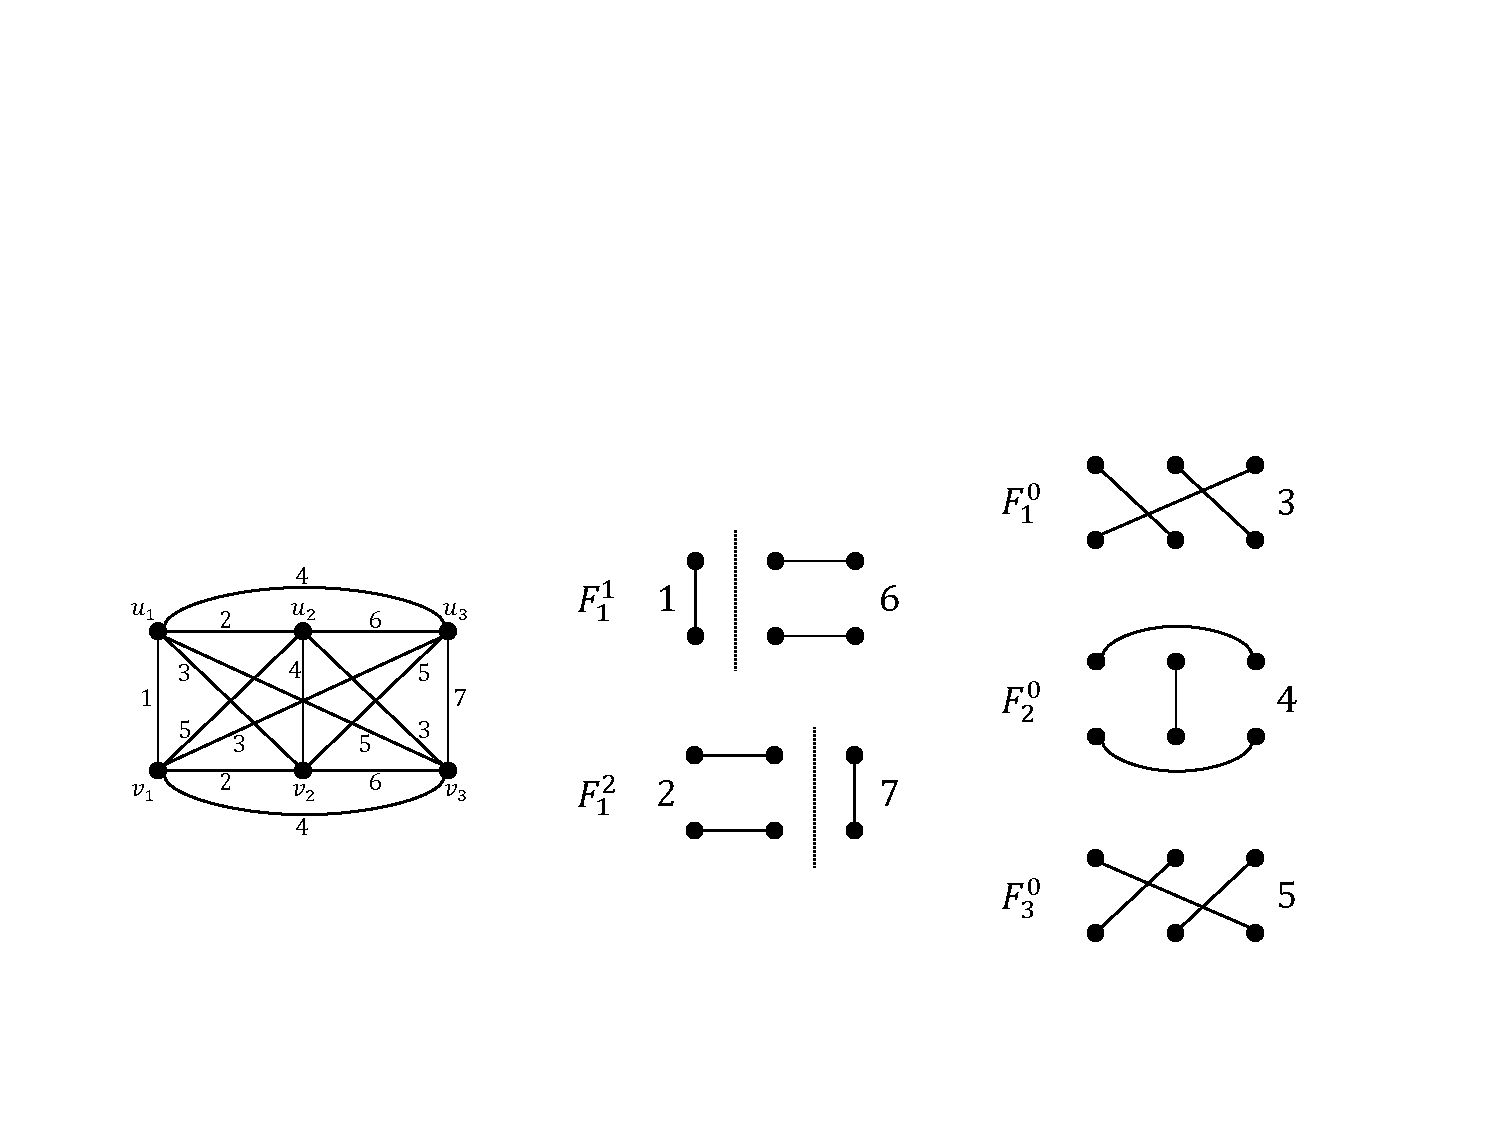
\includegraphics[width=0.8\textwidth]{figures/K_6factorization.pdf}
\label{K_6factorization}
\end{figure}
\end{frame}